\chapter{Introduction} \label{ch01}

\section{Introduction}

Carbon dioxide is a vital part of the earth's ecosystem and makes up approximately 423 ppm (parts per million) of the atmosphere right now (Mauna Loa Observatory, 2024).
Carbon dioxide is made up of two molecules, one carbon molecule and two oxygen atoms, with the oxygen atoms having a double bond with carbon, cancelling the net dipole movement, thus making it a nonpolar gas (Belford, 2016).

This study will discuss how carbon dioxide is used in the manufacture of soft drinks and the effects and behaviours of Le Chatelier's equilibrium within this system; additionally, Trautz and Lewis’s collision theory will be discussed throughout the study.

The process of how carbon dioxide turns into carbonic acid within a carbonated beverage such as Coca-Cola and artificially carbonated waters will be observed.
In addition, the manufacturing process of carbonated soft drinks will be discussed and its impacts on the law, legislation, environment, and socioeconomic aspects of the process.



\chapter{Background Information}\label{ch02}

\section{Background Information}

\subsection{Le Chateliers principle}

Le Chateliers principle is essential for understanding equilibrium equations, and his principle states that a reaction at equilibrium will continue to stay in equilibrium unless an external force causes disturbance, where the system will try to create a new equilibrium state. Le Chatelier had first come up with his principle in 1884 and had later finalised it in 1933 (Lower, 2024).

\begin{center}
    \textit{“If a dynamic equilibrium is disturbed by changing the conditions, the position of equilibrium shifts to counteract the change.” } (Le Chatelier, 1884)
\end{center}

This essentially means that if any factor that affects an equilibrium is altered, the system will adjust to minimise the impact of that change, eventually establishing a new equilibrium.
 The conditions that can cause an equilibrium shift in a system are concentration, temperature, pressure (gas reactions), catalyst’s, and volume changes in a gas system. \\

Le Chatelier states that when the concentration of a reaction is altered, the system will work to return the system back to equilibrium	.
So when a reactant is increased, the forward reaction will be lowered and the equilibrium will be shifted to the right, favouring the reverse reaction. In the opposite reaction, where the product is increased, the reverse reaction will be lowered, shifting the equilibrium to the left, favouring the forward reaction (Davis, Disney, and Smith, 2018). \\

A simplified way to say this is to consider if you were in your room, consider the following: 

\begin{figure}[htp]
    \centering
    \[
        Clean \ Room \rightleftharpoons Messy \ Room
    \]
    \caption{}
    \label{fig:enter-label}
\end{figure}
	

If the room is clean, you might leave your socks and clothes on the floor; in this way, you increase the concentration of messiness in your room, which in turn makes the reverse reaction more favourable where you clean your room, but once your room is clean, the concentration of messiness is lower than the concentration of cleanliness; in turn, you mess up your room again, leading to an equilibrium. (Ihde, 1989). \\

Pressure and temperature also play important roles in the equilibrium of a system. Le Chatelier states that in gaseous reactions, when the pressure is increased, the equilibrium will shift to the side with fewer moles, and when the pressure is decreased, the reverse will happen, where the reaction with more moles is favoured (Davis, Disney, and Smith, 2018). \\

The production of methanol, which includes combining carbon monoxide gas and hydrogen gas, is typically performed under a high pressure (100 atm); this allows for a maximum yield of methanol, making it more suitable for commercial applications. 

\begin{figure}[htp]
    \centering
    \[
       CO (g) + 2H_{2} (g) \rightleftharpoons CH_{3}OH(g) \\
    	\Delta H = -90.7 kJ/mol
    \]
    \caption{}
    \label{fig:enter-label}
\end{figure}

In this reaction, there is a 3:1 ratio of gas molecules, where there is one carbon monoxide molecule and two hydrogen moles to 1 methanol molecule on the right. In this system, if the volume were to decrease by two, the pressure of the system would increase by two in turn. The increased pressure of the system would make it so there are more molecules colliding, favouring the forward reaction with fewer moles until equilibrium is reached. \\

For a system at equilibrium, when temperature is altered, the system would work to go back into equilibrium. Le Chateliers Principle states that when the temperature is increased within a system, the reaction that is endothermic (absorbs heat) will be favoured until the system reaches a state of equilibrium again; when the temperature is decreased within a system, the exothermic (releasing heat) reaction will be favoured until equilibrium is reached again. \\

Consider the following reaction below: 

\begin{figure}[htp]
    \centering
    
    % https://q.uiver.app/#q=WzAsOSxbMCwwLCJOaXRyb2dlbiJdLFswLDEsIlxcYnVsbGV0Il0sWzAsMiwiSHlkcm9nZW4gXFxcXCBGcm9tIFxcIE5hdHVhbCBcXCBHYXMiXSxbMSwwLCJOaXRyb2dlbiBcXCBBbmQgXFwgSHlkcm9nZW4gXFxcXCAxOjMgXFwgUmF0aW8iXSxbMiwxLCJJcm9uIFxcIENhdGFseXN0IFxcXFwgNDAwXm8gQyBcXCAyMDBhdG0iXSxbMiwyLCJHYXMgXFwgY29vbGVkIFxcIHRvIFxcIGZvcm0gXFxcXCBsaXF1aWQgXFwgYW1tb25pYSJdLFsxLDEsIlxcYnVsbGV0Il0sWzIsMywiXFxidWxsZXQiXSxbMSwzLCJcXGJ1bGxldCJdLFswLDFdLFsyLDFdLFsxLDRdLFs0LDVdLFs1LDddLFs3LDgsIlVudXNlZCBcXCBHYXNzZXMgXFwgUmVjeWNsZWQiXSxbOCw2XV0=
    \begin{tikzcd}
	Nitrogen & \begin{array}{c} Nitrogen \ And \ Hydrogen \\ 1:3 \ Ratio \end{array} \\
	\bullet & \bullet & \begin{array}{c} Iron \ Catalyst \\ 400^o C \ 200atm \end{array} \\
	\begin{array}{c} Hydrogen \\ From \ Natual \ Gas \end{array} && \begin{array}{c} Gas \ cooled \ to \ form \\ liquid \ ammonia \end{array} \\
	& \bullet & \bullet
	\arrow[from=1-1, to=2-1]
	\arrow[from=2-1, to=2-3]
	\arrow[from=2-3, to=3-3]
	\arrow[from=3-1, to=2-1]
	\arrow[from=3-3, to=4-3]
	\arrow[from=4-2, to=2-2]
	\arrow["{Unused \ Gasses \ Recycled}", from=4-3, to=4-2]
\end{tikzcd}
    \caption{Production of Ammonia}
    \label{fig:enter-label}
\end{figure}

In this reaction, the forward reaction is exothermic and had a heat enthaply of \begin{math}\Delta H \end{math}. In this reaction, an iron catalyst is combined with potassium hydroxide to increase the efficiency of the reaction; additionally, the pressure that most manufacturing plants use is 200 atm or over. Using Le Chatelier’s Principle, increasing the pressure of a system will favour the reaction that produces the lowest amount of molecules; in the Habes process, the left-hand side of the process has 4 molecules and the right-hand side has 2 molecules. This is used to get the maximum amount of ammonia in the manufacturing process (Clark, 2023)

\subsection{Collision Theory}
Collision theory was first theorised by two chemists, Max Trautz in 1916 and William Lewis in 1918 (Fleming, 2021). Collision theory states that all reactions occur due to particles colliding with each other; this explains why different reactions occur at different rates, as more collisions would lead to a faster reaction (Byjus, 2011). \\
It is stated that for a reaction to occur, it must first collide with another particle, have enough energy to start the reaction (activation energy), and have the proper orientation (Lawson and Lower, 2023).
The most common equation used to calculate the rate of a reaction according to equilibrium theory is: 
\begin{math} Rate = Z_{ab}F \end{math}

In this equation, \begin{math} Rate = Z_{ab}F \end{math} represents the frequency of collisions between molecules A and B, and F is the amount of collisions that will lead to a successful reaction occurring.
Increasing the number of collisions in a system typically increases the rate of reaction. Factors that can influence this are: \\

\subsubsection{Concentration and Volume}
Having a higher concentration of particles within system will lead to more collisions per second. \\

\begin{figure}
    \centering
    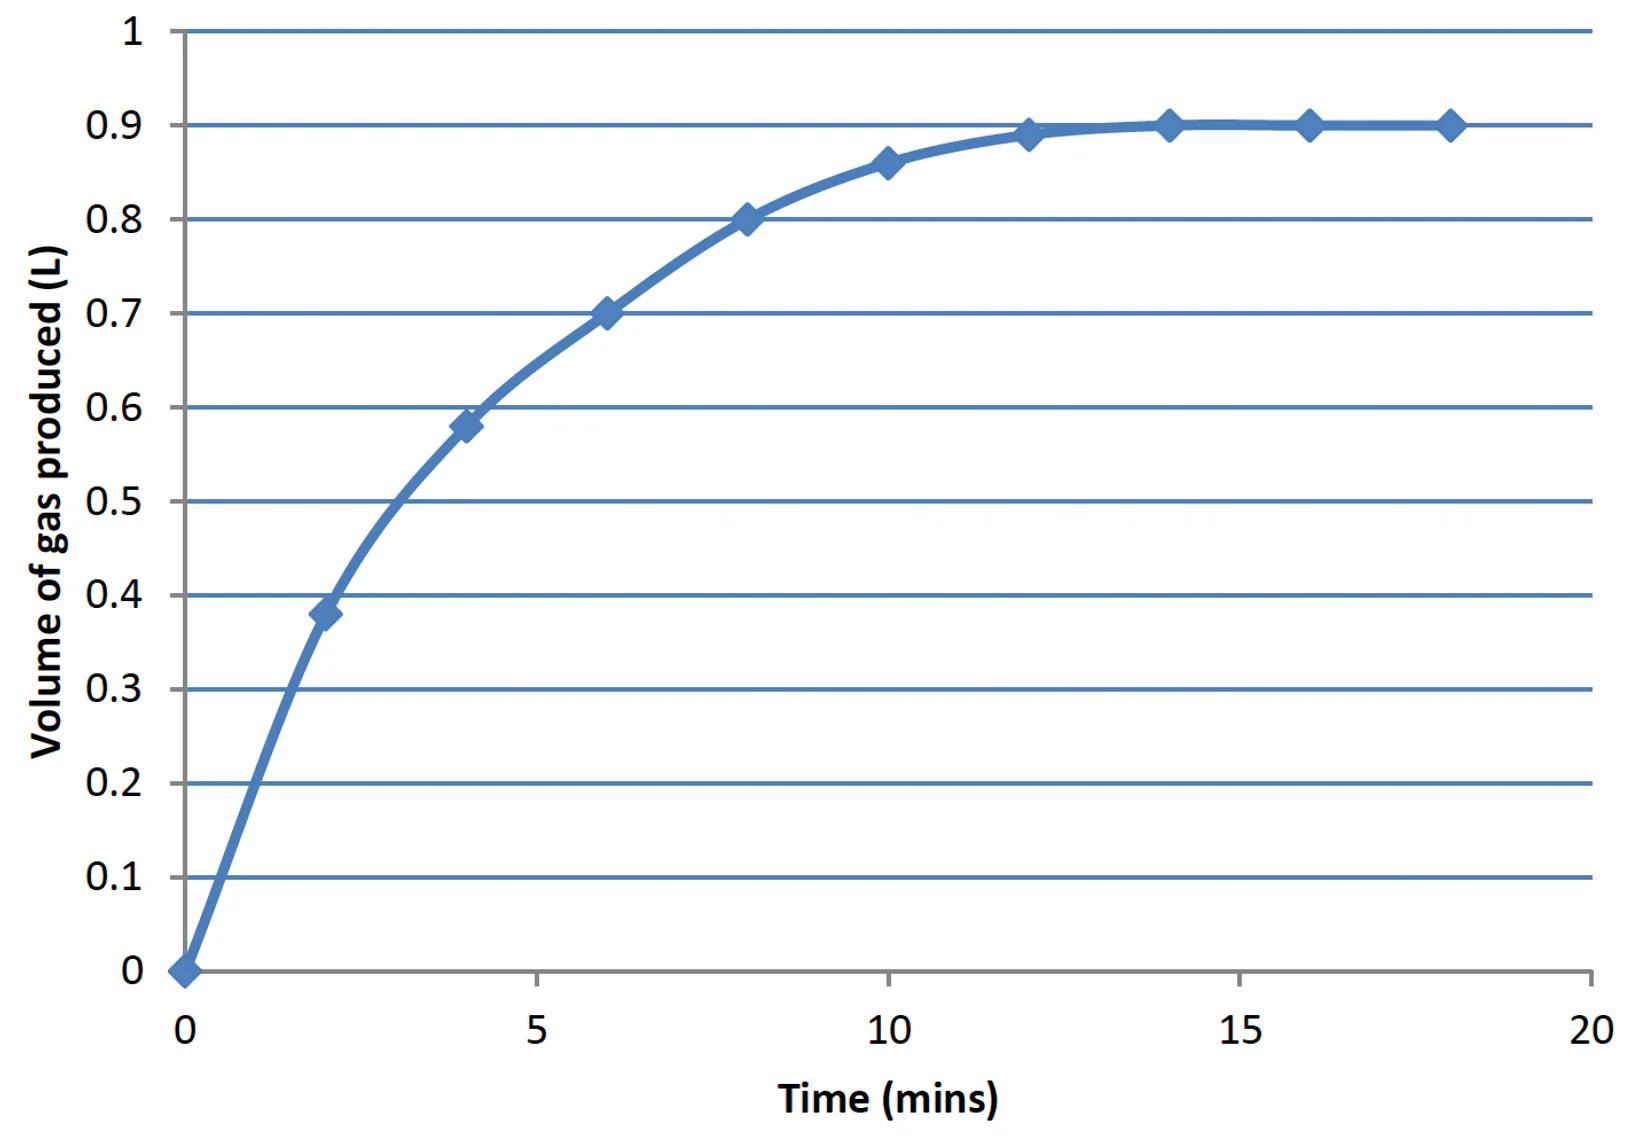
\includegraphics[width=1\linewidth]{assets/1.jpg}
    \caption{As time goes on and more gas is produced, pressure will increase.}
    \label{fig:enter-label}
\end{figure}

As a reaction takes place, the concentration of the reaction will be lowered, leading to fewer reactions, and thus the reaction rate decreases over time, until reaching zero when the limiting reagent is completely used up. \\
Pressure/Volume also increases the rate of reaction in gaseous reactions due to their being less room for the particles to go, so they collide with each other more often in a smaller space (Science Ready, 2019).

\subsubsection{Temperature}
In a system, a higher temperature would lead to a higher kinetic energy of particles; this makes the particles move faster, which leads to them colliding more frequently with higher energy, increasing the reaction rate (Science Ready, 2019).
Kinetic energy energy is given as


\begin{figure}[htp]
    \centering
    \[
         K = 1/2 mv^2 \\
        Where \\
        m = particle mass \\
        v  = speed
    \]
    \caption{}
    \label{fig:enter-label}
\end{figure}

\subsubsection{Surface Area}
Increasing the surface area in a reaction by crushing the reactants into a power, such as iron powder in a thermite reaction, can increase the rate of reaction by allowing more iron to be melted by the reaction. \\
Think of it as having a cup of water. In a cup, the water is only exposed to the top of the cup, and it may be quite small; however, when you spill it across a counter top, the water gets more area in which it can interact and collide with other particles. So which would react faster? putting a block of iron outside to rust or putting iron shavings outside to rust. It would obviously be the iron shavings due to them having a greater surface area when compared to the iron block (Dillon, 2024).

\subsubsection{Catalysts}



\subsubsection{Example}
Consider the following dynamic equilibrium equation: 

\begin{figure}[htp]
    \centering
    \[
        2NO_{2}(g) \rightleftharpoons N_{2}O_{4}(g) \\

	Initial Concentrations \\
	2NO_{2}(g) : 0 mol L^-1	\\ N_{2}O_{4}(g) : 0.5 mol L^-1
    \]
    \caption{}
    \label{fig:enter-label}
\end{figure}

In this reaction, \begin{math}N_{2}O_{4}(g)\end{math} will decompose in its reverse reaction to form \begin{math}NO_{2}(g)\end{math} molecules. Initially the concentration of \begin{math}N_{2}O_{4}(g)\end{math} is high, and this means there are lots of collisions occurring. As time goes on, the forward reaction slows down as more \begin{math}N_{2}O_{4}(g)\end{math} molecules are formed, eventually reaching a dynamic equilibrium where both forward and reverse rates are occurring at the same rate (Scienceready, 2019).

\begin{figure}
    \centering
    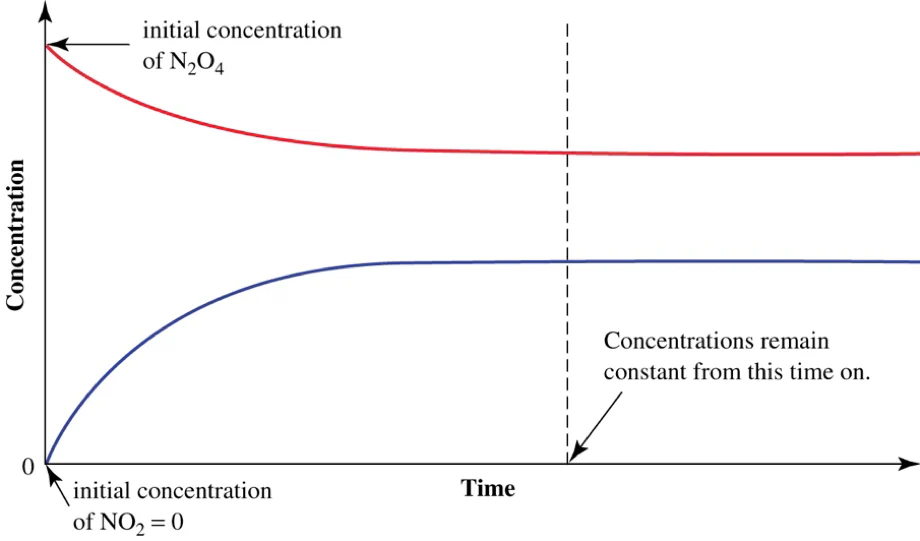
\includegraphics[width=1\linewidth]{2.jpg}
    \caption{Concentration of \begin{math}N_{2}O_{4}\end{math} and \begin{math} NO_{2}\end{math} reaching equilibrium as forward and reverse reactions occur at the same rate.}
    \label{fig:enter-label}
\end{figure}

\subsection{Activation Energy and Reaction Rate}
The law of activation energy, otherwise known as the Arrhenius law, states the minimum kinetic or potential energy needed to stretch, bend, or break bonds to start a chemical reaction. This minimum energy is known as the activation energy and is commonly expressed as \begin{math}E_{a}\end{math} (Bui et al., 2022). //

\begin{figure}
    \centering
    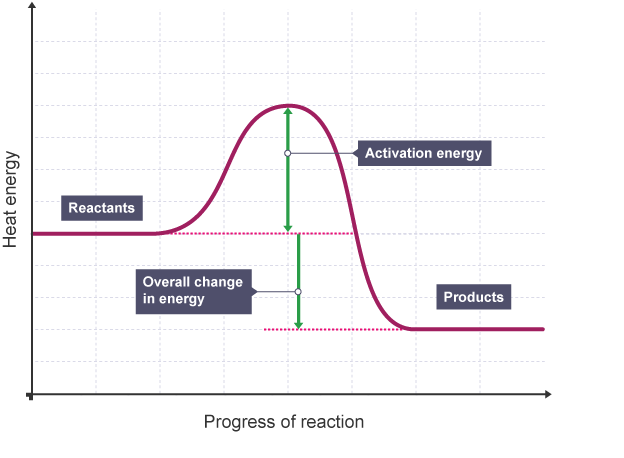
\includegraphics[width=0.5\linewidth]{assets/3.png}
    \caption{Activation energy graph (BBC Bitesize, 2021)}
    \label{fig:enter-label}
\end{figure}

The activation energy (\begin{math}E_{a}\end{math}) is also known as the transition state and is the point at which the most energy is in the system. So if the molecules reacting have an energy higher than the transition state energy, the reaction will continue; this means if a reaction has a very high activation energy, more energy is needed to start the reaction (Bui et al., 2022).

\section{Equilibrium constant}
The equilibrium constant is usually denoted as K, and it provides information about the relationship of products and reactants in a chemical reaction at equilibrium. Equilibrium constant of concentration is denoted as \begin{math}K_{c}\end{math} and is the ratio of the concentration of products to the concentration of the reactants, each raised to their respective stoichiometric coefficients. \\

For a generic reverse reaction equation: 

\begin{figure}[htp]
    \centering
    \[
        aA + bB \rightleftharpoons cC + dD
    \]
    \caption{}
    \label{fig:enter-label}
\end{figure}

The equilibrium constant would be calculated as:

\begin{figure}[htp]
    \centering
    \[
        K_{eq} = \frac{[C]^c \ [D]^d}{[A]^a \ [B]^b} \\ 
        Where: \\
        K > 1 : Products are favoured at equilibrium. \\
        K < 1 : Reactants are favoured at equilibrium. \\
	    K = 1 : Both reactants and products are found at roughly the same amounts.

    \]
    \caption{}
    \label{fig:enter-label}
\end{figure}

However, in a reaction that included gases, the equilibrium constant would be calculated using \begin{math}K_{p}\end{math}, as P is the partial pressure of the system.

\begin{figure}[htp]
    \centering
    \[
        K_{p} = \frac{[P_{C}]^c \ [P_{D}]^d}{[P_{A}]^a \ [P_{B}]^b}
    \]
    \caption{}
    \label{fig:enter-label}
\end{figure}

So in an equilibrium system, the equilibrium constant can be used to see if the forward or reverse reactions are more favourable or if the system has roughly equal parts reactants and products.










\chapter{Discovery and The Manufacture of Soft Drinks}\label{ch3}

\subsection{Some History of Soft Drinks}
The consumption of soft drinks has taken form for many centuries and was initially first used in fermented barley drinks that contained herbs and alcohol to kill any diseases or bacteria in the water, making it safe to drink. As time went on, the first officially marketed soft drink was a drink containing lemon juice with honey (Steen and Ashurst, 2006). Of course at this time the only way to get carbon dioxide within a drink was fermentation of beers and wines; moreover, the push to study carbonated drinks was pushed forward as the natural springs and spas in Holland \& Pyrmont and Seltzer in Germany were known for their therapeutic use. Though the claims for the therapeutic and medicinal properties of carbonated drinks were largely exaggerated, they still had a ‘fizz’ that made the drink more palatable and visually appealing. \\

As the soft drink industry grew, there were more than 50 manufacturers in the 1840’s just in London. Popular carbonated beverage company J.Schweppe \& Co. had paid £5000 for the licence to sell soda and mineral waters at this time, equating to roughly \$355,000 AUD today. \\

\subsection{Discovery of Carbon Dioxide}
Carbon dioxide was one of the first studied gases that was seen as different from regular air. Belgian scientist Jan Baptista van Helmont was one of the first to note the effects of carbon dioxide when he burned charcoal in a closed vessel and noted the difference of mass in the ash and charcoal before. He hypothesised that the rest of the charcoal had transformed into an invisible substance that he named ‘gas silvestre’ (carbon dioxide) (Chastain, 2019). \\
Later, Scottish scientist Joseph Black found that when limestone (calcium carbonate) was heated, it would form a gas he called ‘fixed air’. It was observed that this gas was denser than normal air; we now know that carbon dioxide has a density of \begin{math}1.98 kg/m^3\end{math} at standard conditions. roughly ~1.5 times more dense than air (Univerzita Karlova, 2023), and that this gas could not support animal or plant life (Robert G.W. Anderson, 2019). It was also discovered that when this was bubbled in an aqueous solution of calcium hydroxide (lime), it would form calcium carbonate, making the solution milky, as shown in Fig 3.1 (Smith and Davis, 2017). \\

\begin{figure}[htp]
    \centering
    \[
        Ca(OH)_{2} \ + \ CO_{2} \to CaCO_{3} + H_{2}O \\
        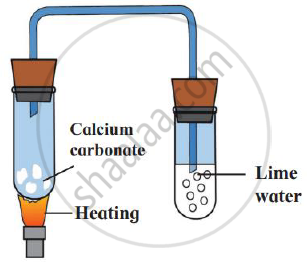
\includegraphics[width=0.5\linewidth]{assets/4.png}
    \]
    \caption{Chemical reaction of lime water and carbon dioxide gas forming calcium carbonate participate.}
    \label{fig:enter-label}
\end{figure}

\subsection{Water Treatment}
Firstly, in the production line of soft drinks, water is sourced, and this water (in Europe) must meet a standard with the EC Drinking Water Directive 80/778/EEC, and if this water is not up to standard, there may be acute or adverse effects over a short or long period of time. Contamination may include, but is not limited to, heavy metal poising, chemical irritant exposure, \& biological hazards such as E. coli or cholera (Directive (EU), 2020).\\
Firstly, the water is passed through tanks that contain sand, filtered gravel, and coarse gravel; this process ensures that the water is free of any foreign mass or organic matter. \\
A common method to disinfect the water of any organisms is by using chlorine and sodium hypochlorite; in this process, 6–8 mg/L of chlorine is added to sterilise the water. At this amount, chlorine will oxidise all impurities, removing taste and odour caused by phenol (used to make plastics, explosives, and drugs such as aspirin) or other similar substances (Wade, 2018) (Griffiths, 2016).
When dissolving chlorine in water, it forms hydrochloric acid and hypochlorous acids. \newline
\begin{center}
    \begin{math}
    Cl_{2} + H_{2}O = HCl + HOCl
\end{math}
\end{center}
\newpage
Due to hypochlorous acid being a weak acid, it dissociates, giving off a hypochlorite ion.

\begin{center}
    \begin{math}
    HOCl = H^{2} + OCl^{-} 
\end{math}
\end{center}


After this process, the sterilised water is then passed through a series of carbon filters, which work to de-chlorinate the solution.
\begin{figure}[htp]
    \centering
    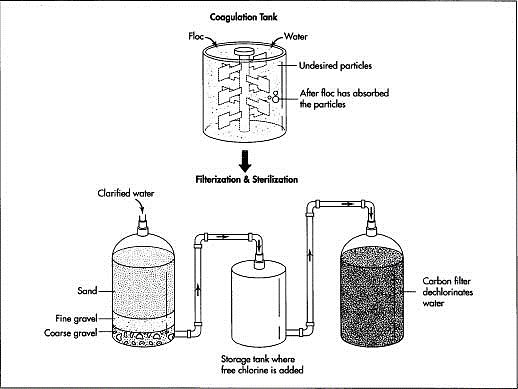
\includegraphics[width=0.5\linewidth]{assets/5.png}
    \caption{Water filter and sterilisation within a manufacturing plant.}
    \label{fig:enter-label}
\end{figure}

\section{Carbonation}
When carbon dioxide is dissolved in water (Fig 3.3 \& 3.4), the solubility of \begin{math}CO_{2}\end{math} varies depending on the surrounding pressure, so when water is carbonated, it is typically kept at 2.04–2.38 atm (30–35 psi) as this makes it so the water is able to dissolve more gas easily (Camp Keg, 2024). The solubility is affected negatively by higher temperatures and is affected positively at higher pressures, at \begin{math}15.5^O C \end{math}and at a pressure of 1 atm. The main purpose of this process is to form carbonic acid (\begin{math}H_{2}CO_{3}\end{math}), which partly dissociates to form bicarbonate and carbonate ions (Steen and Ashurst, 2006). \\

\begin{figure}[htp]
    \centering
    \[
        CO_{2}(g) + H_{2}O(l) \rightleftharpoons H_{2}CO_{3}
    \]
    \caption{Carbon dioxide being dissolved into water forming carbonic acid.}
    \label{fig:enter-label}
\end{figure}

\begin{figure}[htp]
    \centering
    \[
        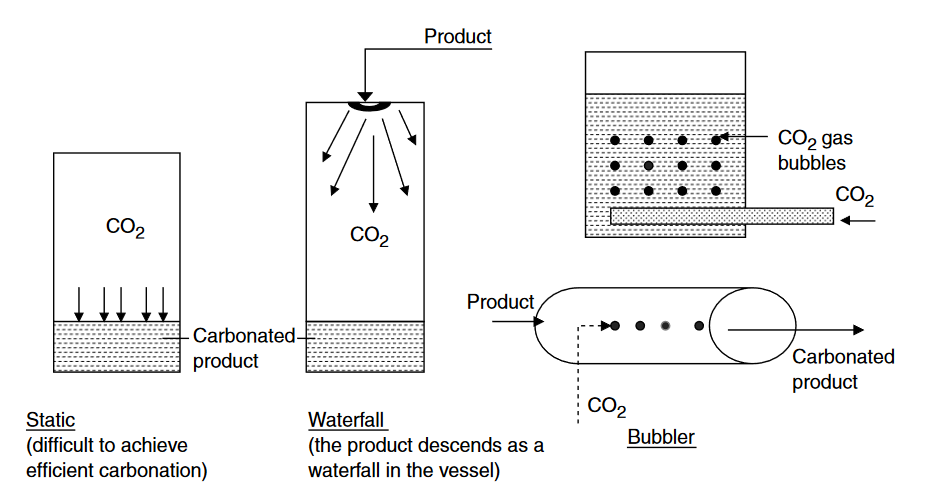
\includegraphics[width=0.5\linewidth]{assets/6.png}
    \]
    \caption{Typical carbonation system (Steen and Ashurst, 2006, p 130).}
    \label{fig:enter-label}
\end{figure}

\newpage

When carbonic acid is formed, it is a diprotic acid that has two hydrogen's that can disassociate into two salts, either hydrogen carbonates (\begin{math}HCO_{3} ^-\end{math} )  or carbonates on their own (\begin{math}CO_{3} ^2-\end{math}) (Britannica, 2019).

\begin{figure}[htp]
    \centering
    \[
        H_{2}CO3 + H_{2}O \rightleftharpoons H_{3}O^+ + HCO_{3}^{\ -} \\
        K_{a1} = 2.5 * 10^{-4} mol/L \ ; \ _{p}K_{a1} = 3.60 \ at \ 25 °C.
    \]
\end{figure}
\begin{figure}[htp]
    \centering
    \[
        HCO_{3}^{-} + H_{2}O \rightleftharpoons H_{3}O^{+} + CO_{3}^{\ 2-} \\
        K_{a2} = 5.61×10^{-11} mol/L \ ; \ _{p}K_{a2} = 10.25 \ at \ 25 °C.
    \]
    \caption{Hydrogen and Carbonates disassociating}
    \label{fig:enter-label}
\end{figure}

The formation of hydrogen ions decreases the pH within the system and makes the overall product acidic.

The standard machinery used for this is the simple in-line carbonator (Fig X), which injects gas bubbles into the liquid in a stream. This process allows more formation of gas bubbles due to the high surface area, leading to more dissolved carbon dioxide gas into the mixture.

\begin{figure}[htp]
    \centering
    \[
        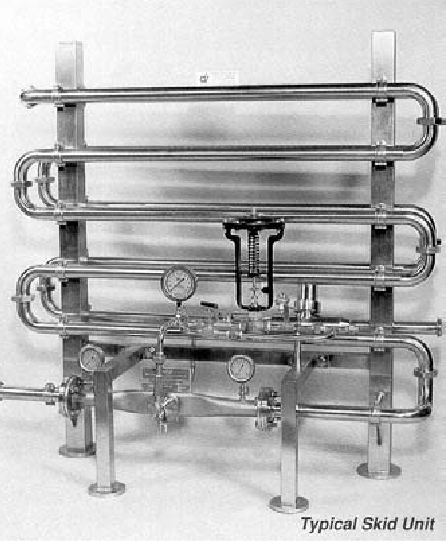
\includegraphics[width=0.5\linewidth]{assets/7.png}
    \]
    \caption{Simple in-line carbonator (Canongate Technology).}
    \label{fig:enter-label}
\end{figure}

\newpage

After this process, the bottle is filled with the carbonated syrup mixture and then fitted with a cap, given adhesive glue, and labelled with the appropriate brand. It is packed within a box and then sold to consumers on the shelves. This process can be seen in the flowchart in Figure 4.1.

\section{But Why These Condition's?}
Using collision theory, we can see why these conditions are more favourable for the production of soft drinks. \\

Firstly, when the pressure is high in the system, more collisions between the \begin{math}CO_{2}\end{math} and water molecules make the formation of carbonic acid (\begin{math}H_{2}CO_{3}\end{math}) more frequent. \\

Secondly, cooling the system will significantly reduce the kinetic energy of the \begin{math}CO_{2}\end{math} molecules; this makes it so that the molecules are more likely to dissolve within the water and not convert back into their gaseous form. \\

Thirdly, Le Chatelier stated in Chapter 2 that when an equilibrium is shifted, it will work its way until equilibrium can be reached again. 
In this system, the dissolution of \begin{math}CO_{2}\end{math} is an exothermic reaction, so lowering the temperature, the equilibrium shifts to the exothermic side, causing more exothermic reactions, increasing the rate at which \begin{math}CO_{2}\end{math} gets dissolved within the solution.

\chapter{Impacts of Soft Drink Manufacturing}\label{ch04}

The manufacturing of soft drinks has had a major impact on the way our society operates, and its legislation has changed numerous times over its inception. This section will be examining how the laws, society, environment, and industry have changed as a reflection of the overall process of producing soft drinks. \\

Standards make sure that the production of soft drinks is the same throughout all manufacturing and processing plants; this makes it so the auditing and inspection of the operational safety, cleanliness, and efficiency is easily monitored.
The ISO (International Standards Organisation) 9001 provides a quality management and assurance system for all customer aspects of a business, such as products, delivery, service, invoicing, and complaints. \\

In addition to the ISO 9001 standard, the ISO 22000 standard is becoming increasingly popular as it combines elements from the ISO 9001 and the hazard analysis and critical control points (HACCP), which emphasises food safety management within the manufacturing process. \\


\begin{landscape}
\begin{figure}
    \[\begin{tikzcd}
	{H_{2}O} && {Water \ Treatment} && \bullet & Sugar \\
	\\
	&&&&& \begin{array}{c} \diamond \\ Syrup \ Preperation \end{array} &&&& Syrup \\
	\\
	&&&&& Proportioner \\
	{CO_{2}} && Carbonator &&& \bullet \\
	&& \bullet \\
	\begin{array}{c} PET \\ Resin \end{array} && 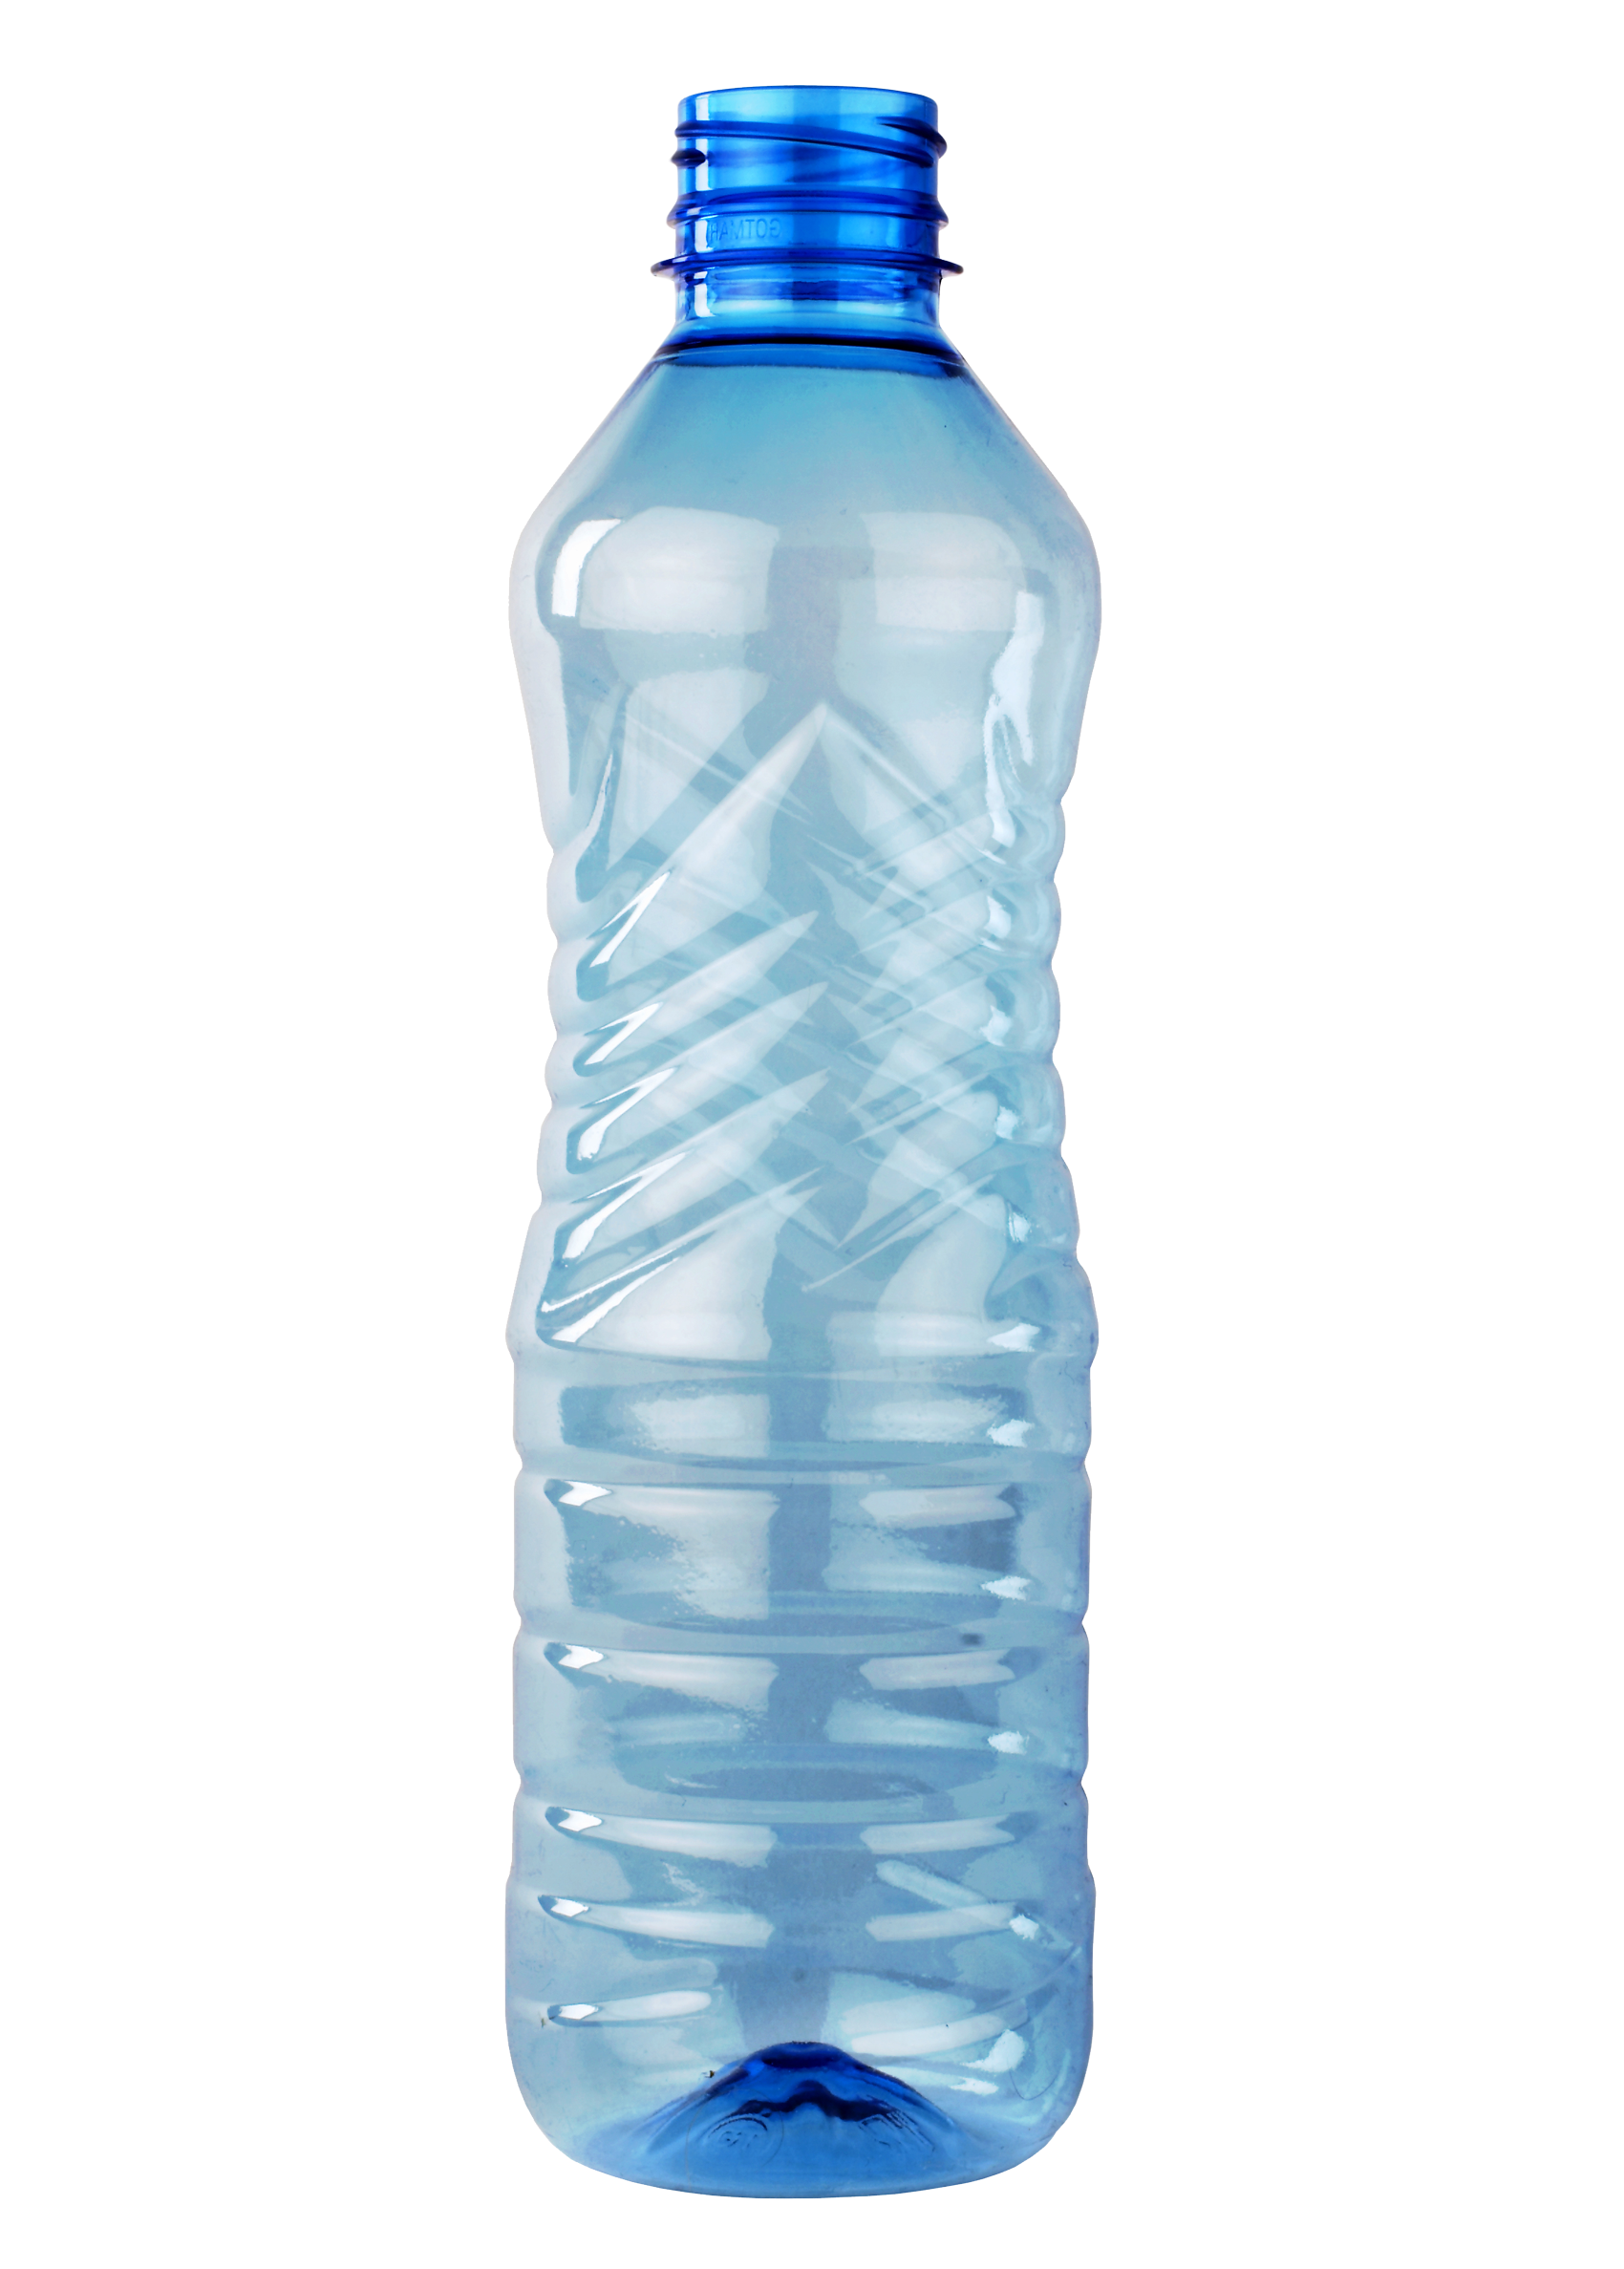
\includegraphics[width=0.03\linewidth]{assets/bottle.png} & 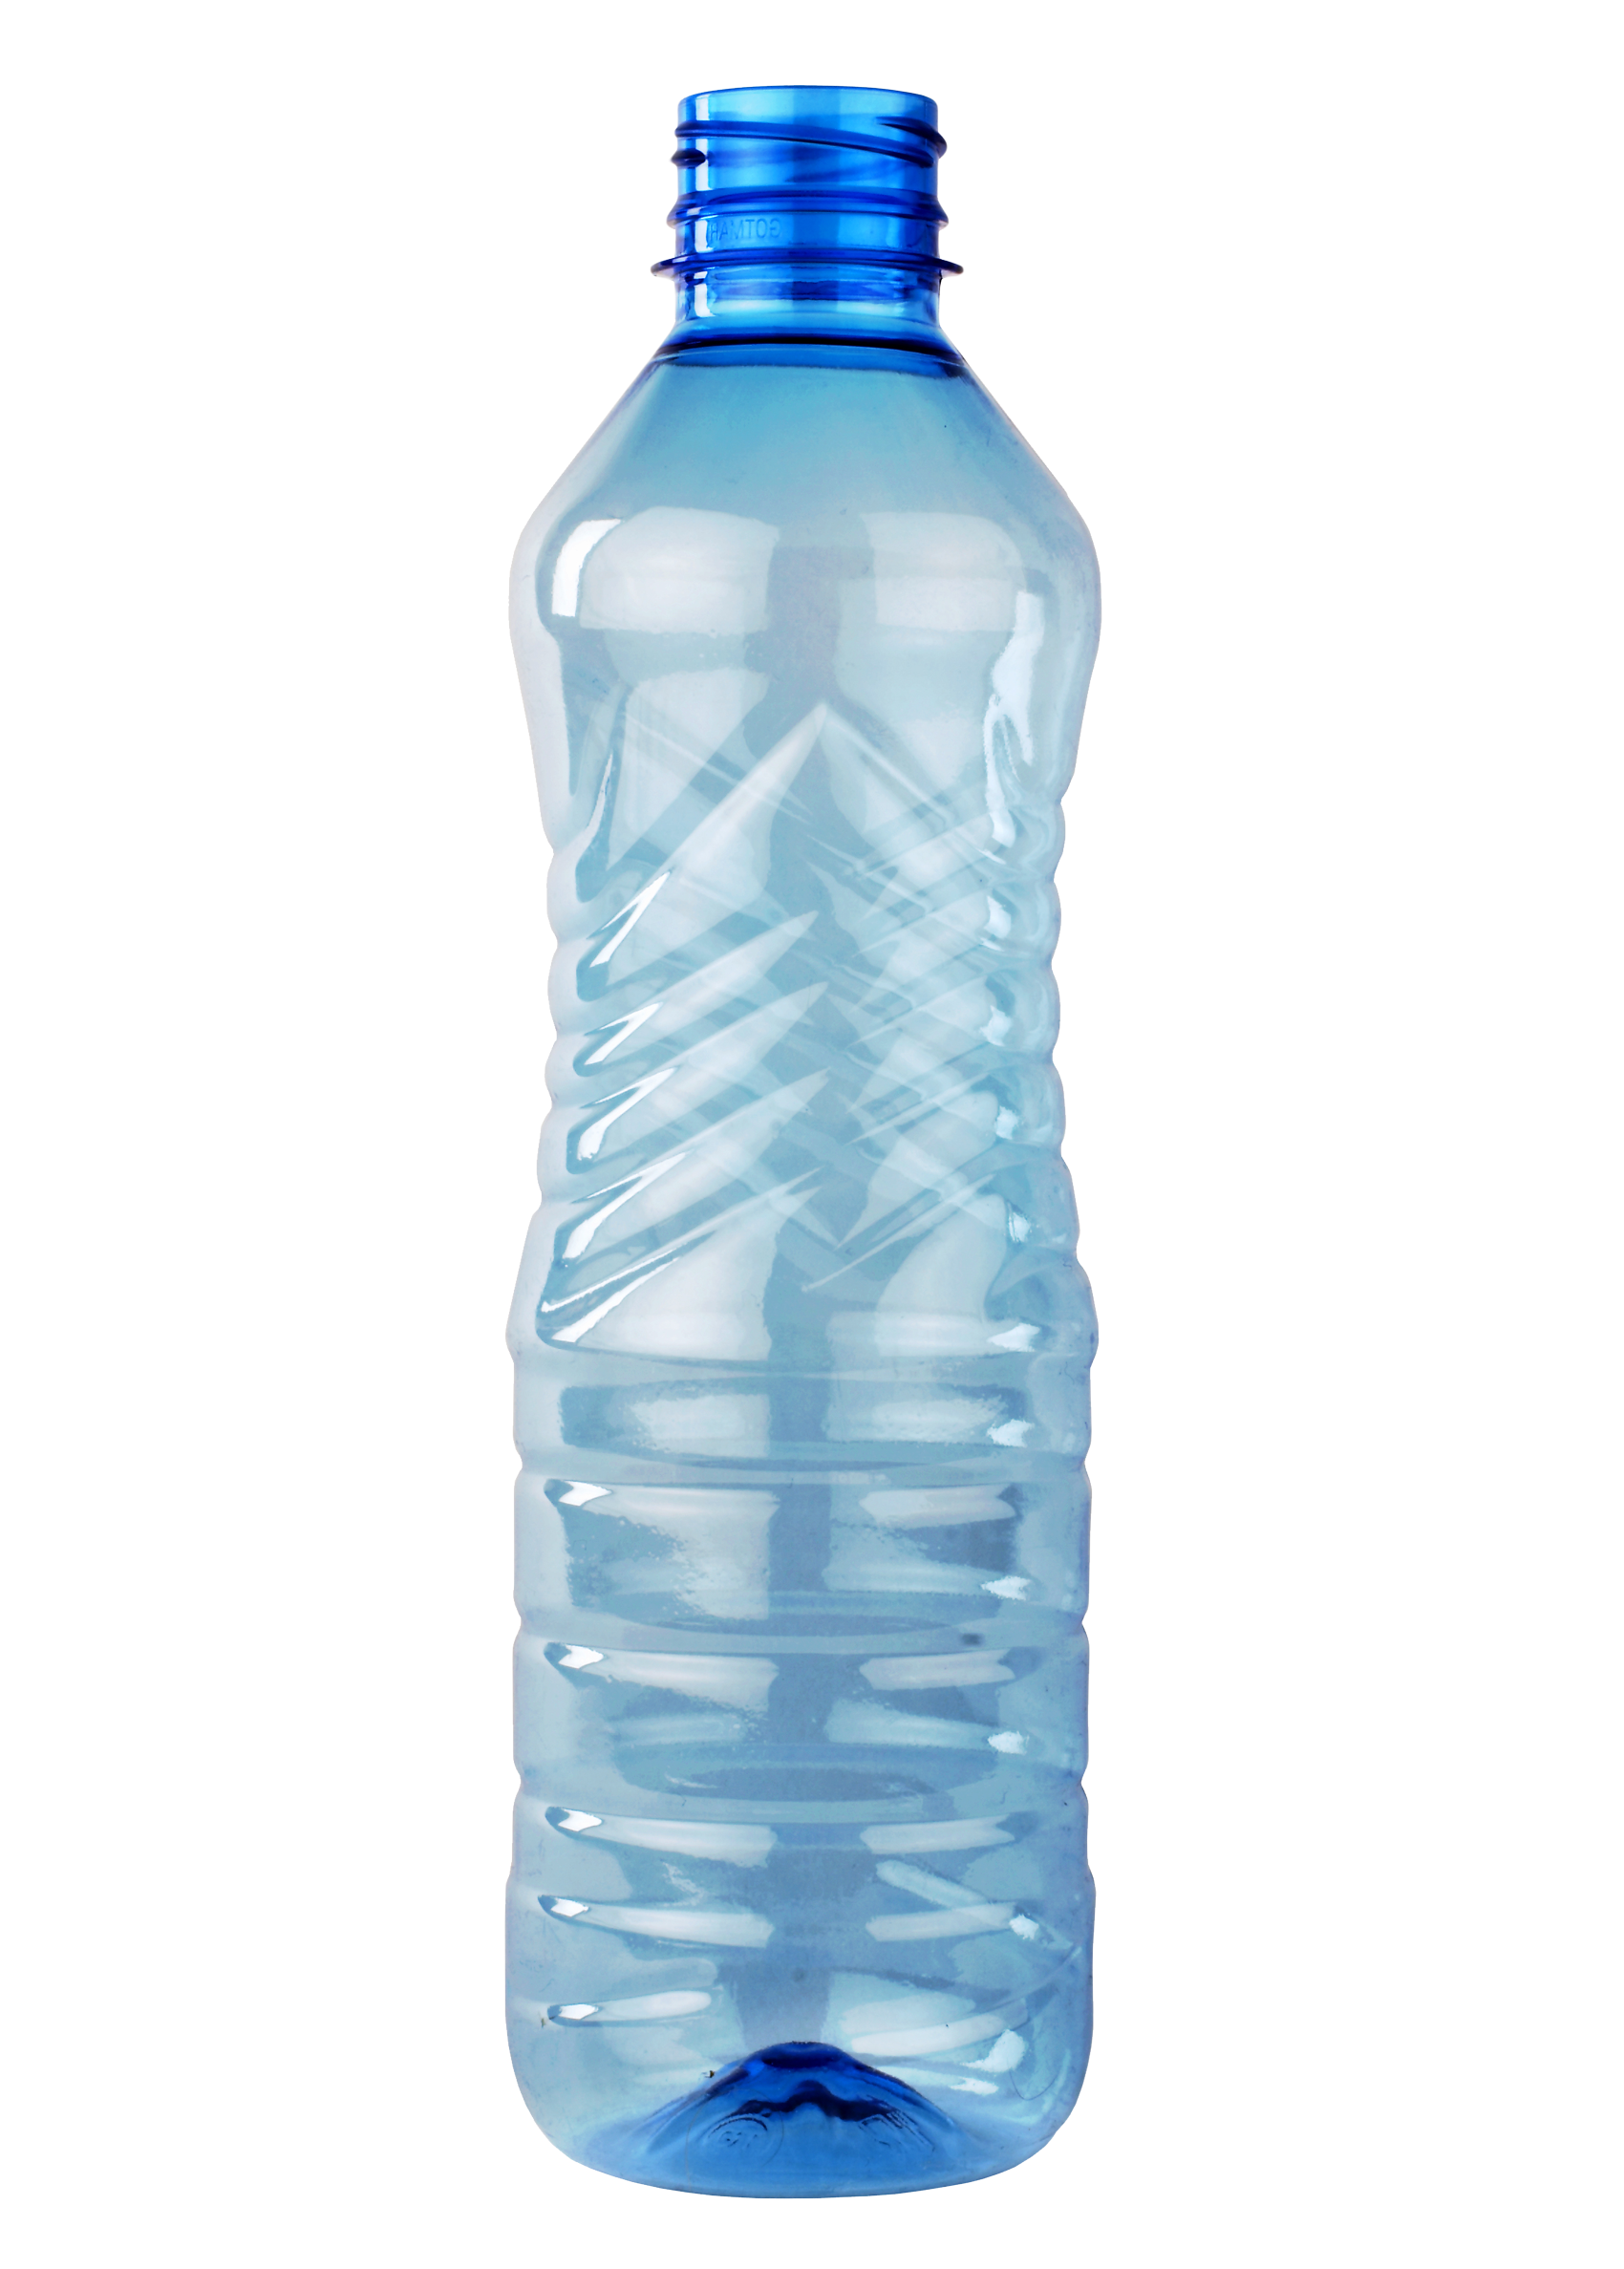
\includegraphics[width=0.03\linewidth]{assets/bottle.png} && 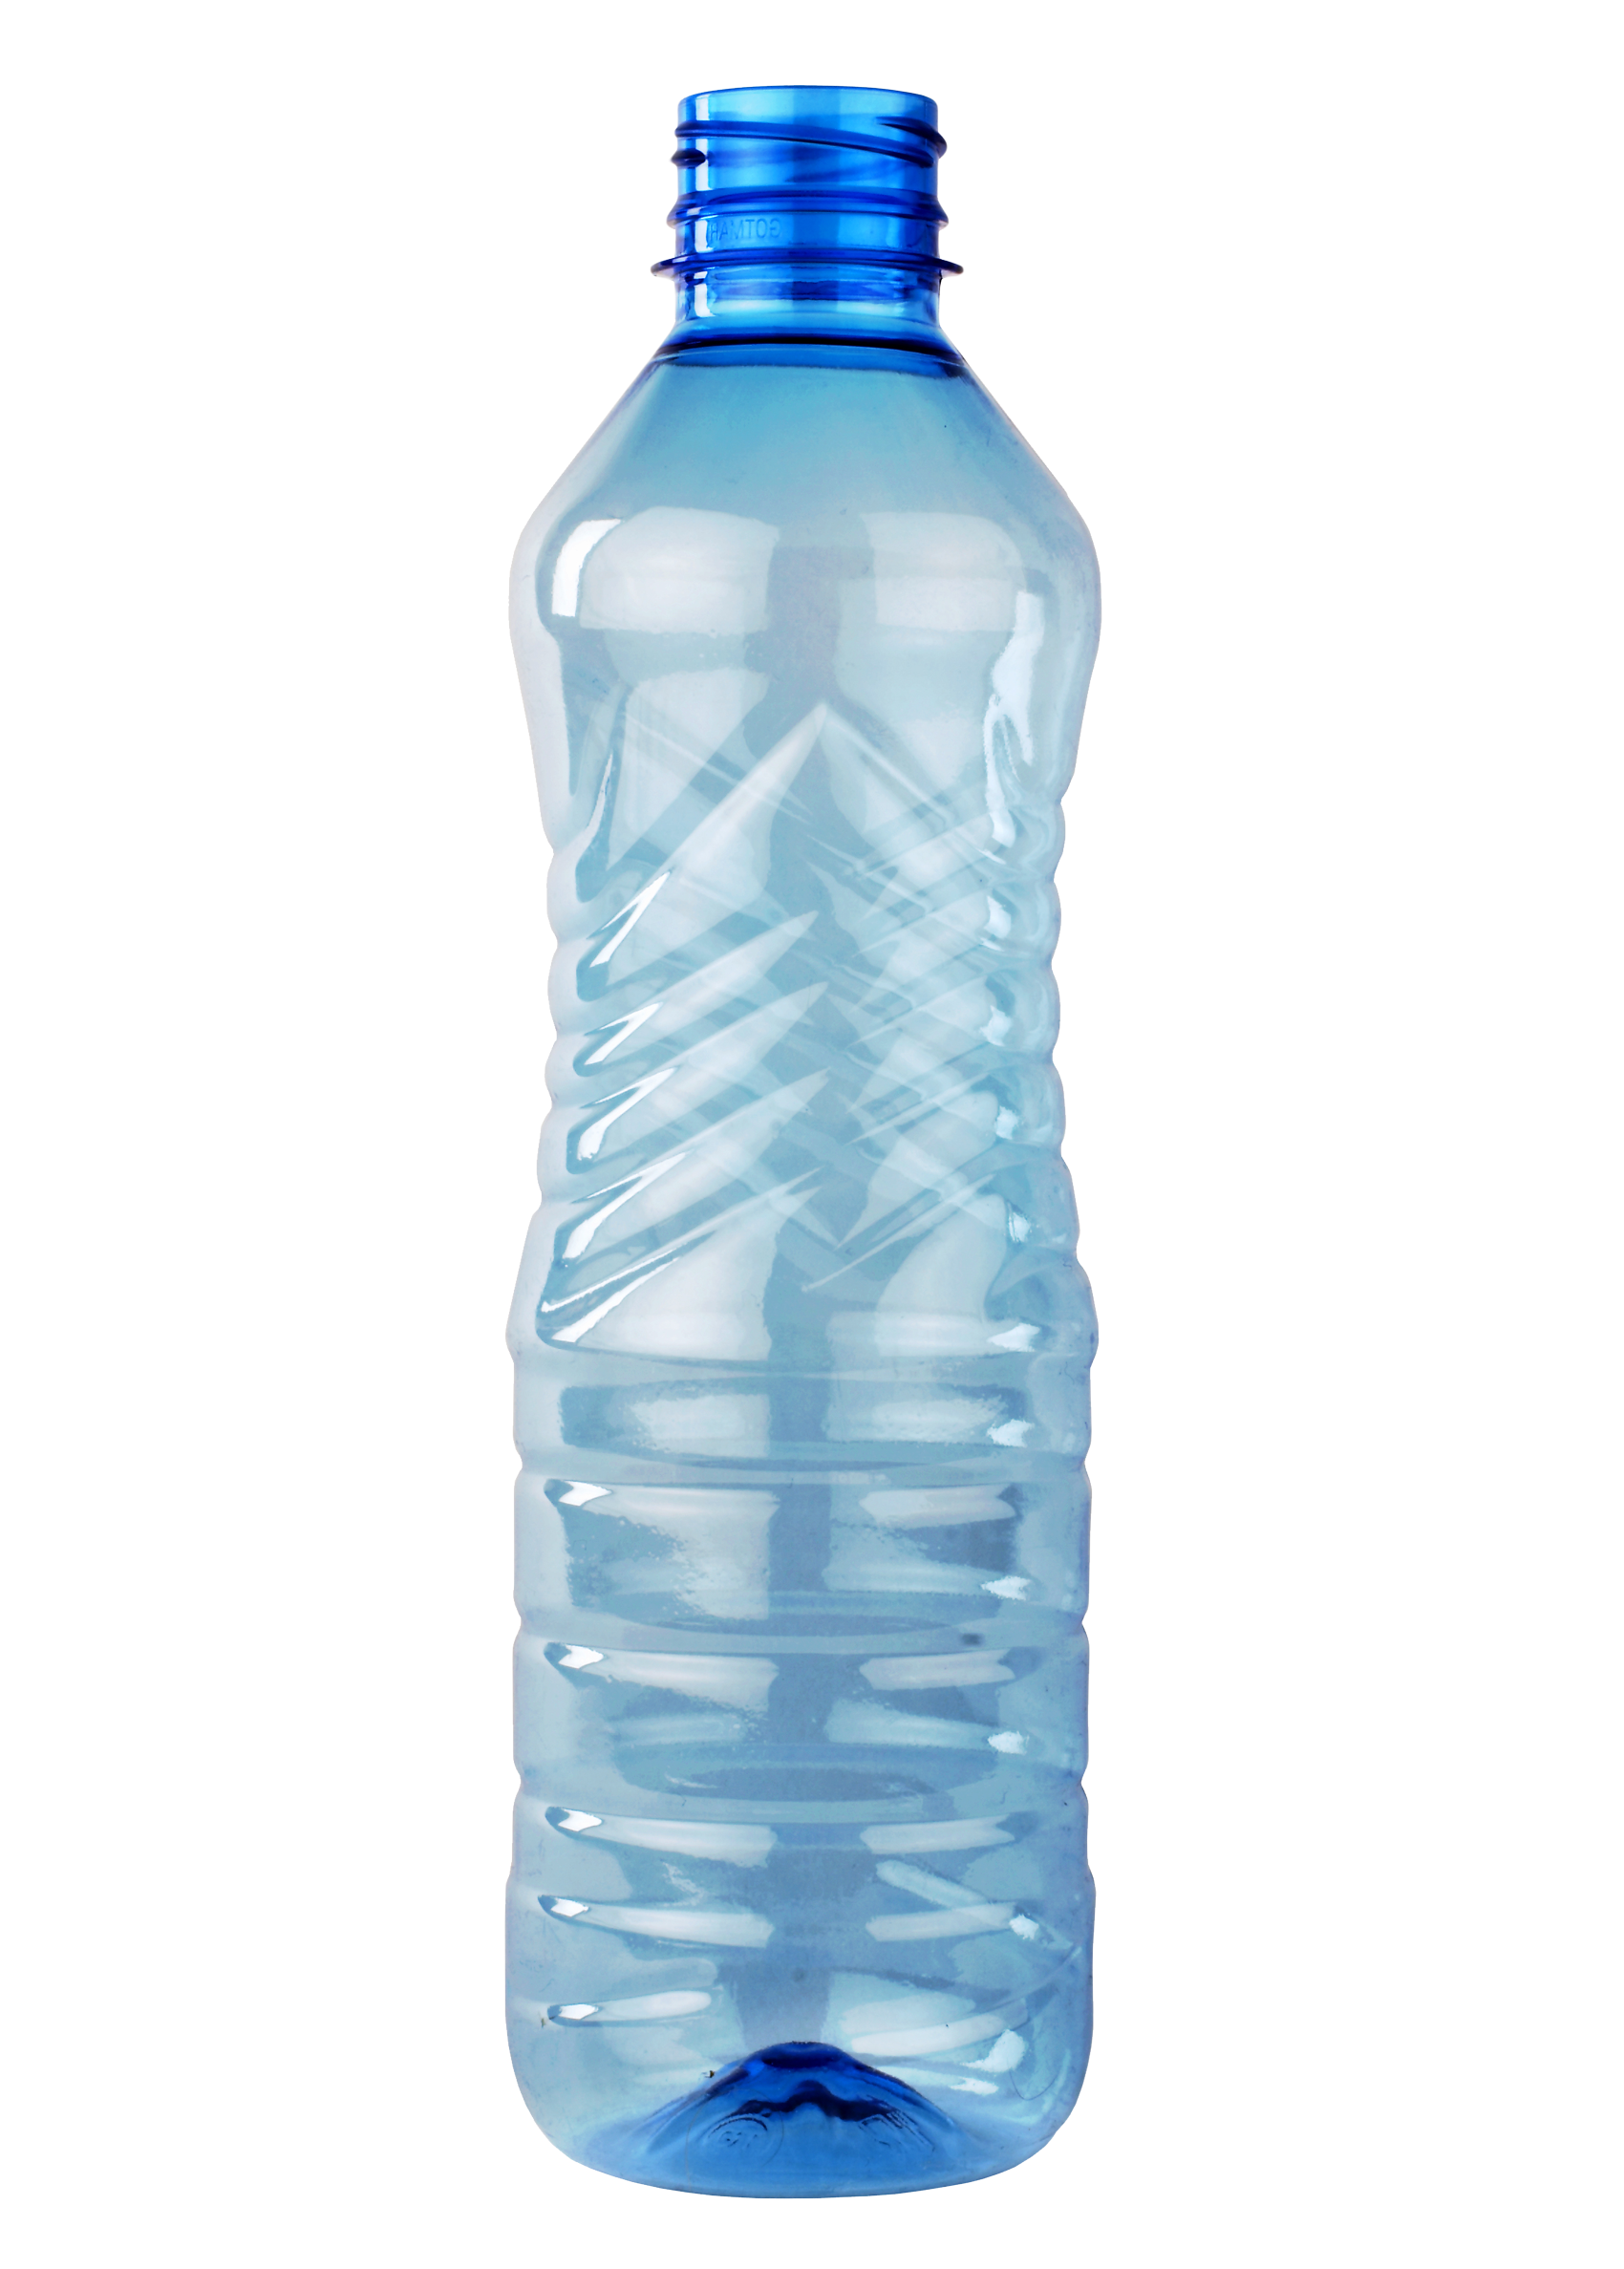
\includegraphics[width=0.03\linewidth]{assets/bottle.png} && 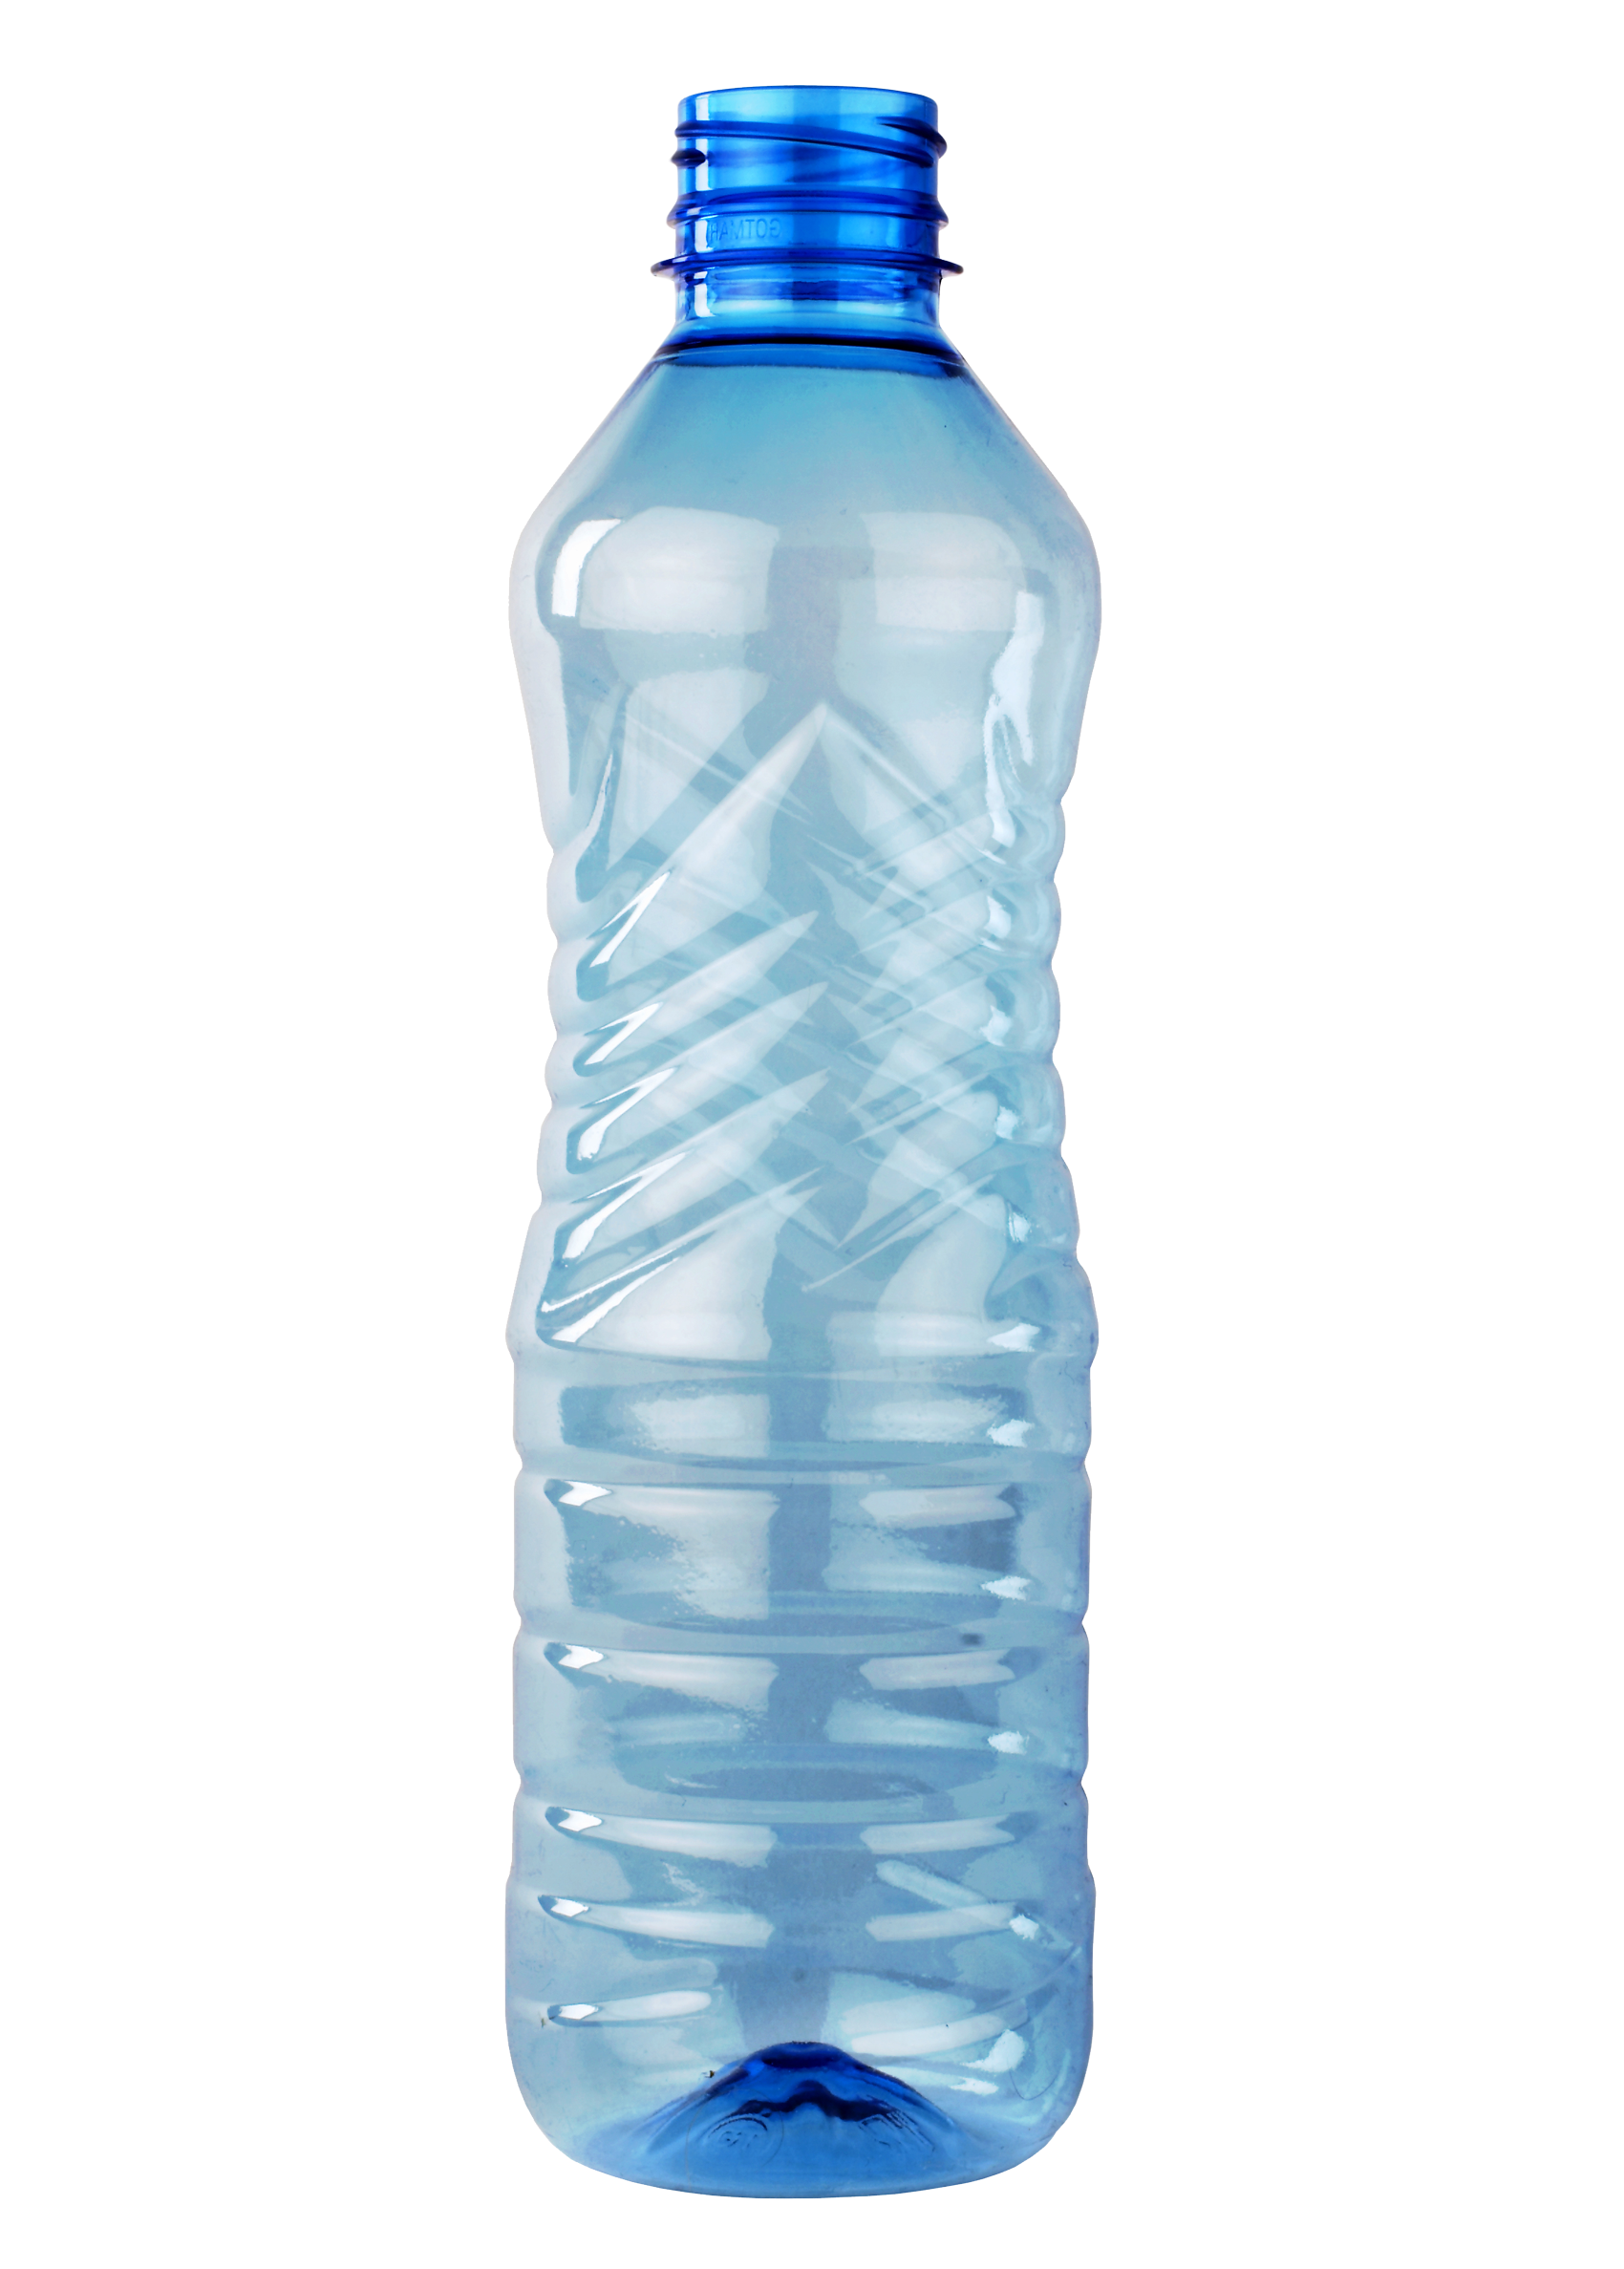
\includegraphics[width=0.03\linewidth]{assets/bottle.png} && 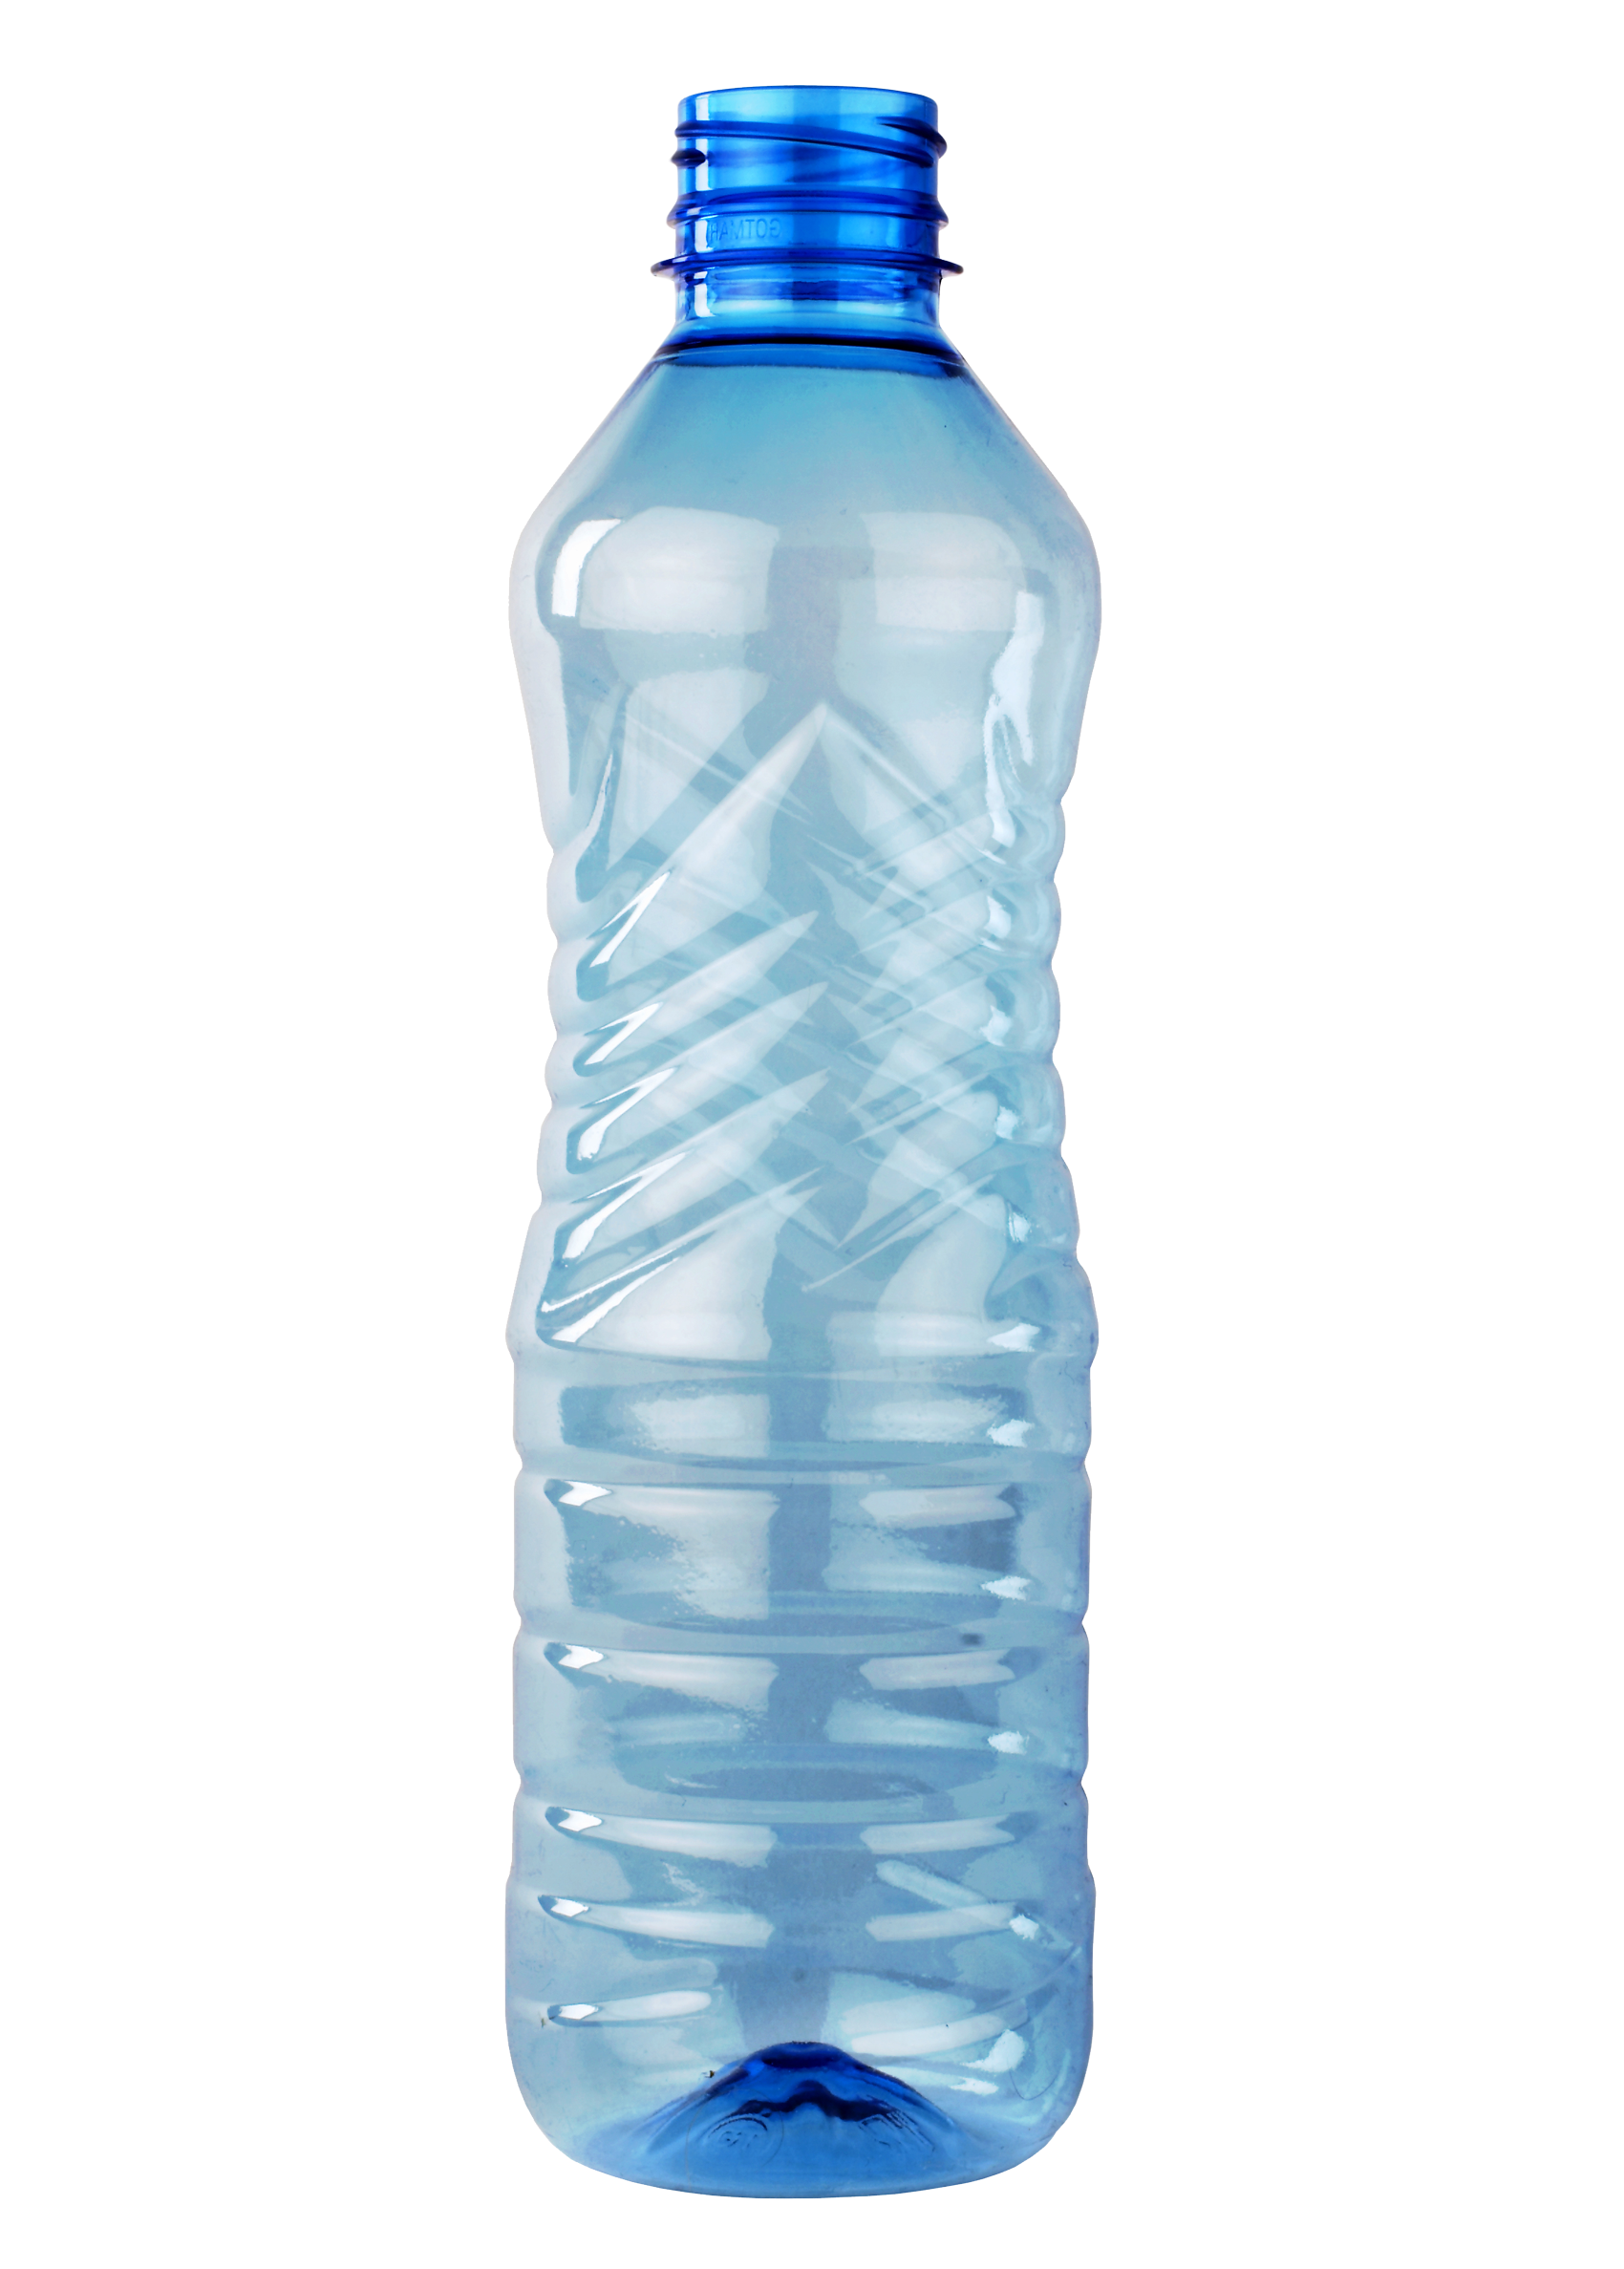
\includegraphics[width=0.03\linewidth]{assets/bottle.png} \\
	&&& \begin{array}{c} CAP \\ (PE) \end{array} && \begin{array}{c} Glue \\ Film (PP) \end{array} && \begin{array}{c} Carton \\ Paper \end{array}
	\arrow[from=1-1, to=1-3]
	\arrow[from=1-3, to=1-5]
	\arrow[from=1-5, to=3-6]
	\arrow[from=1-5, to=5-6]
	\arrow[from=1-6, to=3-6]
	\arrow[from=3-6, to=5-6]
	\arrow[from=3-10, to=3-6]
	\arrow[from=5-6, to=6-6]
	\arrow[from=6-1, to=6-3]
	\arrow["Filler"', from=6-3, to=7-3]
	\arrow[from=6-6, to=6-3]
	\arrow["\begin{array}{c} Bottle \\ Making \end{array}"', from=8-1, to=8-3]
	\arrow[from=8-3, to=8-4]
	\arrow[from=8-4, to=8-6]
	\arrow[from=8-6, to=8-8]
	\arrow["{Final Product}", from=8-8, to=8-10]
	\arrow["Closing", from=9-4, to=8-4]
	\arrow["Labelling", from=9-6, to=8-6]
	\arrow["Packing", from=9-8, to=8-8]
\end{tikzcd}\]
    \caption{Caption}
    \label{fig:enter-label}
\end{figure}
    
\end{landscape}